\textbf{COLUNI 2021 -- Questão 27}\par\medskip Leia a tirinha abaixo.

% COLUNI-AUTO-FIGURES-BEGIN
\begin{figure}[htbp]
\centering
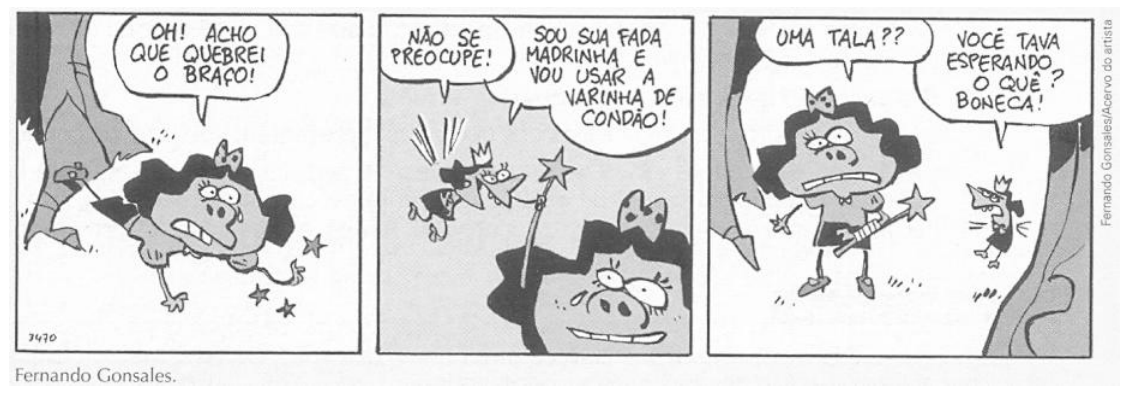
\includegraphics[width=0.95\linewidth]{static/simulados/coluni/figuras/2021/questao-27/figura-1.png}
\end{figure}
% COLUNI-AUTO-FIGURES-END

\par

AGUILAR, João Batista. SIGNORINI, Paula. Ciências Ensino Fundamental 8º Ano, p. 174.

\par

Os ossos do antebraço da personagem fazem parte do sistema esquelético que, em associação aos músculos, possibilita a realização dos movimentos. Com base nas informações apresentadas e nos conhecimentos sobre o assunto, assinale a afirmativa INCORRETA:

\begin{enumerate}
\item O uso de uma tala, em caso de fratura, como na tirinha, ajuda a imobilizar os ossos fraturados até que
       seja realizado tratamento médico adequado.
\item Ossos são órgãos constituídos por tecido ósseo com células vivas, fibras de colágeno, minerais, vasos
       sanguíneos e nervos, o que leva ao risco de sangramento e dor em caso de fratura.
\item Na recuperação de uma fratura é necessária uma alimentação rica em Vitaminas B1 e B2, pois essas
       vitaminas são importantes para o desenvolvimento do tecido ósseo.
\item O hormônio produzido pelas paratireoides atua regulando os níveis de cálcio no sangue, sendo importante
       para o desenvolvimento e a saúde dos ossos.\end{enumerate}
